\documentclass[12pt]{article}
\usepackage[utf8]{inputenc}
\usepackage{amsmath,amsthm,amsfonts,amssymb}
\usepackage{tikz}
\usepackage{subfig}
\usepackage[english]{babel}
\usepackage{capt-of}
\usepackage{tabularray}
\newtheorem{theorem}{Theorem}
\usetikzlibrary{calc}
\usetikzlibrary{shapes}
\usepackage{hyperref}
%might be unnecessary
\usepackage{doi}

%bibliography CMDS

\usepackage{cite}


%%% With amsthm package, creates environments for nicely formatted,
%%% labeled, and numbered propositions, etc.
\theoremstyle{plain}
\newtheorem{thm}{Theorem}
\newtheorem{lemma}[thm]{Lemma}
\newtheorem{prop}[thm]{Proposition}
\newtheorem{conj}[thm]{Conjecture}
\newtheorem{cor}[thm]{Corollary}
\newtheorem{claim}[thm]{Claim}
\newtheorem{fact}[thm]{Fact}

\theoremstyle{definition}
\newtheorem{eg}[thm]{Example}
\newtheorem{defn}[thm]{Definition}
\newtheorem{rem}[thm]{Remark}
\newtheorem{observ}[thm]{Observation}
\newtheorem{open}[thm]{Open Problem}
\newtheorem{prob.}[thm]{Problem}
\newtheorem{quest}[thm]{Question}

% I used these for making definitions and theorems, not what is above
\theoremstyle{remark}
\newtheorem{remark}[thm]{Remark}
\newtheorem{note}[thm]{Note}
\theoremstyle{definition}
\newtheorem{definition}{Definition}[section]
\newtheorem{exmp}{Example}[section]

%personal commands
\newcommand{\cell}[4]{\filldraw[gray!40] ( #1 , #2 ) rectangle ( #3 , #4 ); \draw[thick] ( #1 , #2 ) rectangle ( #3 , #4 );}

\newcommand{\lablnode}[3]{\node[shape=circle,draw=white,fill=white, inner sep=0pt,minimum size=1pt] (A) at ( #1 , #2 ) {\{#3\}};}

%disjoint union symbol code
\makeatletter
\def\moverlay{\mathpalette\mov@rlay}
\def\mov@rlay#1#2{\leavevmode\vtop{%
   \baselineskip\z@skip \lineskiplimit-\maxdimen
   \ialign{\hfil$\m@th#1##$\hfil\cr#2\crcr}}}
\newcommand{\charfusion}[3][\mathord]{
    #1{\ifx#1\mathop\vphantom{#2}\fi
        \mathpalette\mov@rlay{#2\cr#3}
      }
    \ifx#1\mathop\expandafter\displaylimits\fi}
\makeatother

\newcommand{\cupdot}{\charfusion[\mathbin]{\cup}{\cdot}}

%colored cell commands
\newcommand{\cellw}[4]{\draw[thick] ( #1 , #2 ) rectangle ( #3 , #4 );}

\newcommand{\cellred}[4]{\filldraw[red!60] ( #1 , #2 ) rectangle ( #3 , #4 ); \draw[thick] ( #1 , #2 ) rectangle ( #3 , #4 );}

\newcommand{\cellorange}[4]{\filldraw[orange!80] ( #1 , #2 ) rectangle ( #3 , #4 ); \draw[thick] ( #1 , #2 ) rectangle ( #3 , #4 );}

\newcommand{\cellyellow}[4]{\filldraw[yellow!80] ( #1 , #2 ) rectangle ( #3 , #4 ); \draw[thick] ( #1 , #2 ) rectangle ( #3 , #4 );}

\newcommand{\cellgreen}[4]{\filldraw[green!60] ( #1 , #2 ) rectangle ( #3 , #4 ); \draw[thick] ( #1 , #2 ) rectangle ( #3 , #4 );}

\newcommand{\cellpurple}[4]{\filldraw[purple!80] ( #1 , #2 ) rectangle ( #3 , #4 ); \draw[thick] ( #1 , #2 ) rectangle ( #3 , #4 );}

\newcommand{\cellpink}[4]{\filldraw[pink!80] ( #1 , #2 ) rectangle ( #3 , #4 ); \draw[thick] ( #1 , #2 ) rectangle ( #3 , #4 );}

\newcommand{\cellcyan}[4]{\filldraw[cyan!60] ( #1 , #2 ) rectangle ( #3 , #4 ); \draw[thick] ( #1 , #2 ) rectangle ( #3 , #4 );}

\newcommand{\cellblue}[4]{\filldraw[blue!60] ( #1 , #2 ) rectangle ( #3 , #4 ); \draw[thick] ( #1 , #2 ) rectangle ( #3 , #4 );}

\newcommand{\createtri}[6]{\filldraw[gray!40] ( #1 , #2 ) -- ( #3 , #4 ) -- ( #5 , #6 ) -- cycle; \draw[thick] ( #1 , #2 ) -- ( #3 , #4 ) -- ( #5 , #6 ) -- cycle;}

\newcommand{\dimer}[4]{\draw[fill=black] ( #1 , #2 ) circle (3pt);\draw[fill=black] (#3 , #4) circle (3pt);
        \draw[ultra thick] ( #1 , #2 ) -- ( #3 , #4);}
        
\newcommand{\rdimer}[4]{\draw[red,fill=red] ( #1 , #2 ) circle (3pt);\draw[red,fill=red] (#3 , #4) circle (3pt);
        \draw[ultra thick,red] ( #1 , #2 ) -- ( #3 , #4);}
        
\newcommand{\hexagon}{\mathord{\raisebox{0.6pt}{\tikz{\node[draw,scale=.75,regular polygon, regular polygon sides=6](){};}}}}

%nice quick solution
\usepackage[margin=1in]{geometry}
% \usepackage[landscape]{geometry}
\pagenumbering{gobble}
% \usepackage{lscape}

%doc info
\title{Minimal Inscribed Polyforms Summary}
\author{Jack Hanke}

\begin{document}
\maketitle

This document serves as a summary of known enumerations of minimal inscribed polyforms. The rows in each entry correspond with the notation for the family followed by an example polyform. Unless otherwise stated, the size of the example is $n=3$ or $n,m=3,3$. Following this are the first couple terms of the sequence starting at $n=1$ and, if available, the OEIS index. If the sequence has two parameters, the first couple terms are the terms of the main diagonal $n=m$. Finally, the generating function, the $\rho$ function and its domain, and finally any additional notes complete the entry.

\medskip\hrule\medskip
% line 1
$$\square^S_{n,m}$$
\begin{center}
\resizebox{0.15\textwidth}{!}{%
    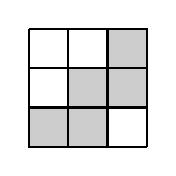
\begin{tikzpicture}
    \draw[step=0.5cm,color=black,thick] (0,0) grid (1.5,1.5);
    \( \cell{0}{0}{0.5}{0.5} \)
    \( \cell{0.5}{0}{1}{0.5} \)
    \( \cell{0.5}{0.5}{1}{1} \)
    \( \cell{1}{0.5}{1.5}{1} \)
    \( \cell{1}{1}{1.5}{1.5} \)
    \end{tikzpicture}
}
\end{center}
$$1, 4, 25, 120, 497, 1924, 7265, \dots (A334551)$$
$$\sum_{n,m \geq 1}\rho(\square^S_{n,m})x^ny^m = \left(1+\frac{xy}{(1-x)(1-y)}\right)^2\frac{2xy}{1-x-y} - \frac{xy}{(1-x)^2(1-y)^2} + \frac{x^2y}{(1-x)^2} + \frac{xy^2}{(1-y)^2}$$
$$\rho(\square^S_{n,m}) = 8\binom{n+m-2}{n-1} -3nm + 2n +2m-8 \text{ for } n,m\geq2$$

Found by Goupil, Cloutier, and Noubound.

\medskip\hrule\medskip
% line 2
$$\triangle^{T}_n$$
\begin{center}
    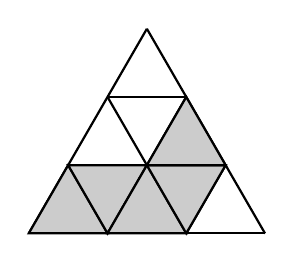
\begin{tikzpicture}
    \newcommand*\rows{3}
    \foreach \row in {0, 1, ...,\rows} {
    \draw[thick] ($\row*(0.5, {0.5*sqrt(3)})$) -- ($(\rows,0)+\row*(-0.5, {0.5*sqrt(3)})$);
    \draw[thick] ($\row*(1, 0)$) -- ($(\rows/2,{\rows/2*sqrt(3)})+\row*(0.5,{-0.5*sqrt(3)})$);
    \draw[thick] ($\row*(1, 0)$) -- ($(0,0)+\row*(0.5,{0.5*sqrt(3)})$);}
    %polyform
    \( \createtri{0}{0}{1}{0}{0.5}{0.866} \);
    \( \createtri{1}{0}{1.5}{0.866}{0.5}{0.866} \);
    \( \createtri{1}{0}{2}{0}{1.5}{0.866} \);
    \( \createtri{2}{0}{2.5}{0.866}{1.5}{0.866} \);
    \( \createtri{1.5}{0.866}{2.5}{0.866}{2}{1.732} \);
    \end{tikzpicture}
\end{center}

$$1, 3, 12, 44, 144, 432, 1216, \dots (A356888)$$
$$\sum_{n\geq1}\rho(\triangle^{T}_n)x^n = \frac{x-3x^2+6x^3}{(1-2x)^3}$$
$$\rho(\triangle^{T}_n) = ((n-1)^2 +2)2^{n-2} \text{ for } n\geq 1$$

\medskip\hrule\medskip
% line 3
$$\triangle^{H}_n$$
\begin{center}
    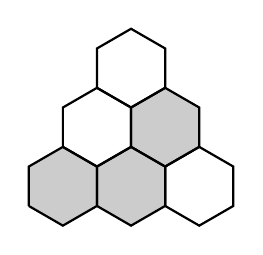
\begin{tikzpicture}
    %polyform
    \filldraw[gray!40] (0,0.25) -- (0.433,0) -- (0.866,0.25) -- (1.299,0) -- (1.732,0.25) -- (1.732,0.75) -- (2.165,1) -- (2.165,1.5) -- (1.732,1.75) -- (1.299,1.5) -- (1.299,1) -- (0.866,0.75) -- (0.433,1) -- (0,0.75) -- (0,0.25);
    \draw[thick] (0,0.25) -- (0.433,0) -- (0.866,0.25) -- (0.866,0.75) -- (0.433,1) -- (0,0.75) -- (0,0.25);
    \draw[thick] (0.866,0.25) -- (1.299,0) -- (1.732,0.25) -- (1.732,0.75) -- (1.299,1) -- (0.866,0.75) -- (0.866,0.25);
    \draw[thick] (1.732,0.25) -- (2.165,0) -- (2.598,0.25) -- (2.598,0.75) -- (2.165,1) -- (1.732,0.75) -- (1.732,0.25);
    \draw[thick] (0.433,1) -- (0.866,0.75) -- (1.299,1) -- (1.299,1.5) -- (0.866,1.75) -- (0.433,1.5) -- (0.433,1);
    \draw[thick] (1.299,1) -- (1.732,0.75) -- (2.165,1) -- (2.165,1.5) -- (1.732,1.75) -- (1.299,1.5) -- (1.299,1);
    \draw[thick] (0.866,1.75) -- (1.299,1.5) -- (1.732,1.75) -- (1.732,2.25) -- (1.299,2.5) -- (0.866,2.25) -- (0.866,1.75);
    \end{tikzpicture}
\end{center}

$$1, 3, 10, 32, 96, 272, 736, \dots (A104270)$$
$$\sum_{n\geq1}\rho(\triangle^{H}_n)x^n = \frac{x-3x^2+4x^3}{(1-2x)^3}$$
$$\rho(\triangle^{H}_n) = \left( \binom{n}{2}+2 \right) 2^{n-2} \text{ for } n\geq 1$$

\medskip\hrule\medskip
% line 4
$$\triangle^{R}_n$$
\begin{center}
    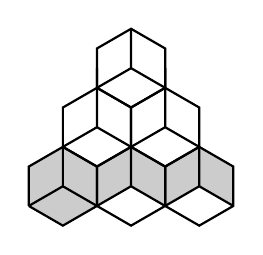
\begin{tikzpicture}
    %polyform
    \filldraw[gray!40] (0,0.25) -- (0.433,0) -- (0.866,0.25) -- (0.866,0.75) -- (0.433,1) -- (0,0.75) -- (0,0.25);
    \filldraw[gray!40] (0.866,0.25) -- (1.299,0.5) -- (1.299,1) -- (0.866,0.75) -- (0.866,0.25);
    \filldraw[gray!40] (1.732,0.25) -- (1.299,0.5) -- (1.299,1) -- (1.732,0.75) -- (1.732,0.25);
    \filldraw[gray!40] (1.732,0.25) -- (2.165,0.5) -- (2.165,1) -- (1.732,0.75) -- (1.732,0.25);
    \filldraw[gray!40] (2.598,0.25) -- (2.165,0.5) -- (2.165,1) -- (2.598,0.75) -- (2.598,0.25);
    %lattice
    \draw[thick] (0,0.25) -- (0.433,0) -- (0.866,0.25) -- (0.866,0.75) -- (0.433,1) -- (0,0.75) -- (0,0.25);
    \draw[thick] (0.866,0.25) -- (1.299,0) -- (1.732,0.25) -- (1.732,0.75) -- (1.299,1) -- (0.866,0.75) -- (0.866,0.25);
    \draw[thick] (1.732,0.25) -- (2.165,0) -- (2.598,0.25) -- (2.598,0.75) -- (2.165,1) -- (1.732,0.75) -- (1.732,0.25);
    \draw[thick] (0,0.25) -- (0.433,0.5) -- (0.433,1) -- (0.433,0.5) -- (0.866,0.25);
    \draw[thick] (0.866,0.25) -- (1.299,0.5) -- (1.299,1) -- (1.299,0.5) -- (1.732,0.25);
    \draw[thick] (1.732,0.25) -- (2.165,0.5) -- (2.165,1) -- (2.165,0.5) -- (2.598,0.25);
    \draw[thick] (0.433,1) -- (0.866,0.75) -- (1.299,1) -- (1.299,1.5) -- (0.866,1.75) -- (0.433,1.5) -- (0.433,1);
    \draw[thick] (1.299,1) -- (1.732,0.75) -- (2.165,1) -- (2.165,1.5) -- (1.732,1.75) -- (1.299,1.5) -- (1.299,1);
    \draw[thick] (0.433,1) -- (0.866,1.25) -- (0.866,2) -- (0.866,1.25) -- (1.299,1);
    \draw[thick] (1.299,1) -- (1.732,1.25) -- (1.732,2) -- (1.732,1.25) -- (2.165,1);
    \draw[thick] (0.866,1.75) -- (1.299,1.5) -- (1.732,1.75) -- (1.732,2.25) -- (1.299,2.5) -- (0.866,2.25) -- (0.866,1.75);
    \draw[thick] (0.866,1.75) -- (1.299,2) -- (1.299,2.5) -- (1.299,2) -- (1.732,1.75);
    \end{tikzpicture}
\end{center}

$$1, 6, 24, 80, 240, 672, 1792, \dots (A001788)$$
$$\sum_{n\geq1}\rho(\triangle^{R}_n)x^n = \frac{x}{(1-2x)^3}$$
$$\rho(\triangle^{R}_n) = n(n+1)2^{n-2} \text{ for } n\geq 1$$

\medskip\hrule\medskip
% line 5
$$\triangle^{K}_n$$
\begin{center}
    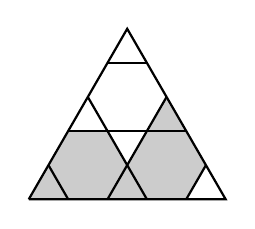
\begin{tikzpicture}
        %polyform
        \filldraw[gray!40] (0,0) -- (0.5,0) -- (0.25,0.433) -- cycle;
        \filldraw[gray!40] (1,0) -- (1.5,0) -- (1.25,0.433) -- cycle;
        \filldraw[gray!40] (1.5,0.866) -- (2,0.866) -- (1.75,1.299) -- cycle;
        
        \filldraw[gray!40] (0.25,0.433) -- (0.5,0) -- (1,0) -- (1.25, 0.433) -- (1,0.866) -- (0.5,0.866) -- (0.25,0.433);
        \filldraw[gray!40] (1.25,0.433) -- (1.5,0) -- (2,0) -- (2.25, 0.433) -- (2,0.866) -- (1.5,0.866) -- (1.25,0.433);
        
        %lattice
        \draw[thick] (0,0) -- (2.5,0) -- (1.25, 2.165) -- (0,0);
        \draw[thick] (1,1.732) -- (1.5,1.732);
        \draw[thick] (0.5,0) -- (0.25,0.433);
        \draw[thick] (2,0) -- (2.25,0.433);
        \draw[thick] (1,0) -- (1.75,1.299);
        \draw[thick] (1.5,0) -- (0.75,1.299);
        \draw[thick] (0.5,0.866) -- (2,0.866);
        \end{tikzpicture}
\end{center}

$$1, 3, 21, 125, 693, 3669, 18733, \dots (A356889)$$
$$\sum_{n\geq1}\rho(\triangle^{K}_n)x^n = \frac{x-10x^2+42x^3-80x^4+56x^5}{(1-x)(1-4x)^3}$$
$$\rho(\triangle^{K}_n) = \left( n^2 + 3n +\frac{10}{3} \right) 4^{n-3} - \frac{1}{3} \text{ for } n\geq 2$$

The above results can be extended by adding $a-2$ additional edges in a symmetric manner, shown below in the labelled dual graph.

$$\triangle^{K,a}_n$$

\begin{center}
    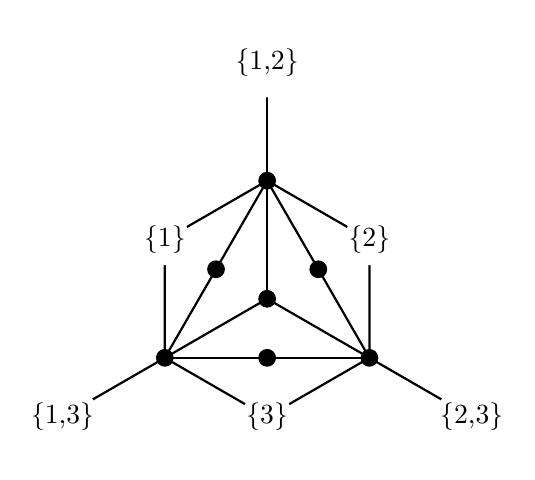
\begin{tikzpicture}
    %edges
    \draw[thick] (0,0) -- (1.299,0.75);
    \draw[thick] (5.196,0) -- (3.897,0.75);
    \draw[thick] (2.598,3) -- (2.598,4.5);
    
    \draw[thick] (1.299,0.75) -- (2.598,0) -- (3.897,0.75) -- (3.897,2.25) -- (2.598,3) -- (1.299,2.25) -- (1.299,0.75);
    \draw[thick] (1.299,0.75) -- (2.598, 1.5) -- (3.897,0.75);
    \draw[thick] (2.598,3) -- (2.598, 1.5);
    % (1.299,0.75) and (2.598,3) gives (1.949,1.875)
    % (3.897,0.75) and (2.598,3) gives (3.248,1.875)
    % (1.299,0.75) and (3.897,0.75) gives (2.598,0.75)
    \draw[thick] (1.299,0.75) -- (1.949,1.875) -- (2.598,3);
    
    \draw[thick] (3.897,0.75) -- (3.248,1.875) -- (2.598,3);
    
    \draw[thick] (1.299,0.75) -- (2.598,0.75) -- (3.897,0.75);
    
    
    %nodes
    \( \lablnode{0}{0}{1,3} \)
    \( \lablnode{2.598}{0}{3} \)
    \draw[fill=black] (1.299,0.75) circle (3pt);
    \( \lablnode{1.299}{2.25}{1} \)
    \draw[fill=black] (3.897,0.75) circle (3pt);
    \( \lablnode{5.196}{0}{2,3} \)
    \( \lablnode{3.897}{2.25}{2} \)
    \draw[fill=black] (2.598,3) circle (3pt);
    \( \lablnode{2.598}{4.5}{1,2} \)
    \draw[fill=black] (2.598,1.5) circle (3pt);
    
    \draw[fill=black] (1.949,1.875) circle (3pt);
    \draw[fill=black] (3.248,1.875) circle (3pt);
    \draw[fill=black] (2.598,0.75) circle (3pt);
    
    \end{tikzpicture}
\end{center}

$$\rho(\triangle^{K,a}_n) = \left(n^2+\frac{(6a^2-5a-5)n}{a+1} + \frac{6(a^4-2a^3+2a+1)}{(a+1)^2}\right)2^{n-2}a^{n-4}-\frac{3(a-1)^n}{(a+1)^2} \text{ for } n\geq 2$$

Interestingly, though initially defined for $a \geq 2$, $\rho(\triangle^{K,1}_n) =  ((n-1)^2  + 2)2^{n-2} = \rho(\triangle^{T}_n)$. So in the case of minimal inscribed polyforms $\triangle^{T}_n$ can be seen as the $a=1$ case of $\triangle^{K,a}_n$.
 
\medskip\hrule\medskip
% line 6
$$\triangle^{H*}_n$$
\begin{center}
    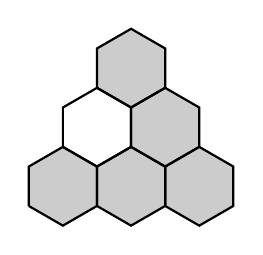
\begin{tikzpicture}
    %polyform
    \filldraw[gray!40] (0,0.25) -- (0.433,0) -- (0.866,0.25) -- (1.299,0) -- (1.732,0.25) -- (1.732,0.75) -- (2.165,1) -- (2.165,1.5) -- (1.732,1.75) -- (1.299,1.5) -- (1.299,1) -- (0.866,0.75) -- (0.433,1) -- (0,0.75) -- (0,0.25);
    \filldraw[gray!40] (1.732,0.25) -- (2.165,0) -- (2.598,0.25) -- (2.598,0.75) -- (2.165,1) -- (1.732,0.75) -- (1.732,0.25);
    \filldraw[gray!40] (0.866,1.75) -- (1.299,1.5) -- (1.732,1.75) -- (1.732,2.25) -- (1.299,2.5) -- (0.866,2.25) -- (0.866,1.75);
    %lattice
    \draw[thick] (0,0.25) -- (0.433,0) -- (0.866,0.25) -- (0.866,0.75) -- (0.433,1) -- (0,0.75) -- (0,0.25);
    \draw[thick] (0.866,0.25) -- (1.299,0) -- (1.732,0.25) -- (1.732,0.75) -- (1.299,1) -- (0.866,0.75) -- (0.866,0.25);
    \draw[thick] (1.732,0.25) -- (2.165,0) -- (2.598,0.25) -- (2.598,0.75) -- (2.165,1) -- (1.732,0.75) -- (1.732,0.25);
    
    \draw[thick] (0.433,1) -- (0.866,0.75) -- (1.299,1) -- (1.299,1.5) -- (0.866,1.75) -- (0.433,1.5) -- (0.433,1);
    \draw[thick] (1.299,1) -- (1.732,0.75) -- (2.165,1) -- (2.165,1.5) -- (1.732,1.75) -- (1.299,1.5) -- (1.299,1);
    
    \draw[thick] (0.866,1.75) -- (1.299,1.5) -- (1.732,1.75) -- (1.732,2.25) -- (1.299,2.5) -- (0.866,2.25) -- (0.866,1.75);
    \end{tikzpicture}
\end{center}

$$1, 1, 3, 11, 41, 153, 573, \dots (A281593)$$
$$\sum_{n\geq1}\rho(\triangle^{H*}_n)x^n = \frac{x-2x^2}{(1-x)\sqrt{1-4x}}$$
$$\rho(\triangle^{H*}_n) = \binom{2(n-1)}{n-1} - \sum_{k=0}^{n-2}\binom{2k}{k} \text{ for } n\geq 1$$

\medskip\hrule\medskip
% line 7
$$\triangle^{T*}_n$$
\begin{center}
    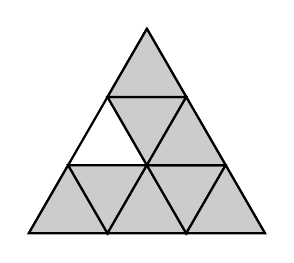
\begin{tikzpicture}
    \newcommand*\rows{3}
    \foreach \row in {0, 1, ...,\rows} {
    \draw[thick] ($\row*(0.5, {0.5*sqrt(3)})$) -- ($(\rows,0)+\row*(-0.5, {0.5*sqrt(3)})$);
    \draw[thick] ($\row*(1, 0)$) -- ($(\rows/2,{\rows/2*sqrt(3)})+\row*(0.5,{-0.5*sqrt(3)})$);
    \draw[thick] ($\row*(1, 0)$) -- ($(0,0)+\row*(0.5,{0.5*sqrt(3)})$);}
    %polyform
    \( \createtri{0}{0}{1}{0}{0.5}{0.866} \);
    \( \createtri{1}{0}{1.5}{0.866}{0.5}{0.866} \);
    \( \createtri{1}{0}{2}{0}{1.5}{0.866} \);
    \( \createtri{2}{0}{2.5}{0.866}{1.5}{0.866} \);
    \( \createtri{2}{0}{3}{0}{2.5}{0.866} \);
    \( \createtri{1.5}{0.866}{2}{1.732}{1}{1.732} \);
    \( \createtri{1.5}{0.866}{2.5}{0.866}{2}{1.732} \);
    \( \createtri{1}{1.732}{2}{1.732}{1.5}{2.598} \);
    \end{tikzpicture}
\end{center}

$$1, 3, 9, 29, 99, 351, 1275 \dots (A006134)$$
$$\sum_{n\geq1}\rho(\triangle^{T*}_n)x^n = \frac{x}{(1-x)\sqrt{1-4x}}$$
$$\rho(\triangle^{T*}_n) = \text{ for } n\geq 1$$

Both $\rho(\triangle^{T*}_n)$ and $\rho(\triangle^{H*}_n)$ rely on the following identity.

\begin{theorem}
    $$\sum_{k_1+k_2+k_3=n}\binom{k_1+k_2}{k_1}\binom{k_2+k_3}{k_2}\binom{k_3+k_1}{k_3} = \sum_{k=0}^n \binom{2k}{k}$$
\end{theorem}

\begin{proof}
    TODO
\end{proof}

\medskip\hrule\medskip
% line 8
$$R^{\theta}_{n,m}$$
\begin{center}
\resizebox{0.2\textwidth}{!}{%
    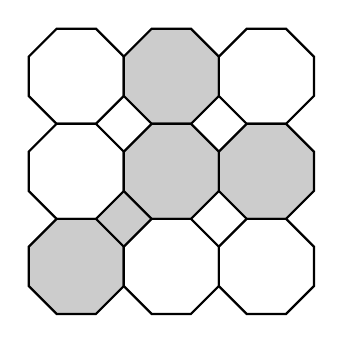
\begin{tikzpicture}
    %polyform
    \filldraw[gray!40](0.0,0.3535) -- (0.3535,0.0) -- 
            (0.8535,0.0) -- (1.207,0.3535) -- 
            (1.207,0.8535) -- (0.8535,1.207) -- 
            (0.3535,1.207) -- (0.0,0.8535) -- cycle;
    \filldraw[gray!40] (1.207,1.5605) -- (1.5605,1.207) -- 
            (2.0605,1.207) -- (2.414,1.5605) -- 
            (2.414,2.0605) -- (2.0605,2.414) -- 
            (1.5605,2.414) -- (1.207,2.0605) -- cycle;     
    \filldraw[gray!40] (1.207,2.7675) -- (1.5605,2.414) -- 
            (2.0605,2.414) -- (2.414,2.7675) -- 
            (2.414,3.2675) -- (2.0605,3.621) -- 
            (1.5605,3.621) -- (1.207,3.2675) -- cycle;
    \filldraw[gray!40] (2.414,1.5605) -- (2.7675,1.207) -- 
            (3.2675,1.207) -- (3.621,1.5605) -- 
            (3.621,2.0605) -- (3.2675,2.414) -- 
            (2.7675,2.414) -- (2.414,2.0605) -- cycle;
            
    \filldraw[gray!40] (1.207,0.8535) -- (0.8535,1.207) -- (1.207,1.5605) -- (1.5605,1.207) -- cycle;

    %lattice
    \draw[thick] (0.0,0.3535) -- (0.3535,0.0) -- 
        (0.8535,0.0) -- (1.207,0.3535) -- 
        (1.207,0.8535) -- (0.8535,1.207) -- 
        (0.3535,1.207) -- (0.0,0.8535) -- cycle;
    \draw[thick] (0.0,1.5605) -- (0.3535,1.207) -- 
        (0.8535,1.207) -- (1.207,1.5605) -- 
        (1.207,2.0605) -- (0.8535,2.414) -- 
        (0.3535,2.414) -- (0.0,2.0605) -- cycle;
    \draw[thick] (0.0,2.7675) -- (0.3535,2.414) -- 
        (0.8535,2.414) -- (1.207,2.7675) -- 
        (1.207,3.2675) -- (0.8535,3.621) -- 
        (0.3535,3.621) -- (0.0,3.2675) -- cycle;
    \draw[thick] (1.207,0.3535) -- (1.5605,0.0) -- 
        (2.0605,0.0) -- (2.414,0.3535) -- 
        (2.414,0.8535) -- (2.0605,1.207) -- 
        (1.5605,1.207) -- (1.207,0.8535) -- cycle;
    \draw[thick] (1.207,1.5605) -- (1.5605,1.207) -- 
        (2.0605,1.207) -- (2.414,1.5605) -- 
        (2.414,2.0605) -- (2.0605,2.414) -- 
        (1.5605,2.414) -- (1.207,2.0605) -- cycle;
    \draw[thick] (1.207,2.7675) -- (1.5605,2.414) -- 
        (2.0605,2.414) -- (2.414,2.7675) -- 
        (2.414,3.2675) -- (2.0605,3.621) -- 
        (1.5605,3.621) -- (1.207,3.2675) -- cycle;       
    \draw[thick] (2.414,0.3535) -- (2.7675,0.0) -- 
        (3.2675,0.0) -- (3.621,0.3535) -- 
        (3.621,0.8535) -- (3.2675,1.207) -- 
        (2.7675,1.207) -- (2.414,0.8535) -- cycle;
    \draw[thick] (2.414,1.5605) -- (2.7675,1.207) -- 
        (3.2675,1.207) -- (3.621,1.5605) -- 
        (3.621,2.0605) -- (3.2675,2.414) -- 
        (2.7675,2.414) -- (2.414,2.0605) -- cycle;
    \draw[thick] (2.414,2.7675) -- (2.7675,2.414) -- 
        (3.2675,2.414) -- (3.621,2.7675) -- 
        (3.621,3.2675) -- (3.2675,3.621) -- 
        (2.7675,3.621) -- (2.414,3.2675) -- cycle;
    \end{tikzpicture}
}
\end{center}

$$1, 6, 43, 256, 1201, 7510, 40363, \dots$$
$$\sum_{n,m\geq1}\rho(R^{\theta}_{n,m})x^n y^m= \left(1+\frac{xy}{(1-x)(1-y)}\right)^2\frac{2xy}{1-x-y-xy} - \frac{xy}{(1-x)^2(1-y)^2} + \frac{x^2y}{(1-x)^2} + \frac{xy^2}{(1-y)^2}$$
$$\rho(R^{\theta}_{n,m}) = 2D(n-1,m-1) - nm + 2 \sum_{i=0}^{n-2}\sum_{j=0}^{m-2}D(i,j)(2+(n-2-i)(m-2-j)) \text{ for } n,m\geq 2$$

\medskip\hrule\medskip
% line 9
$$A^{S^*}_{n,m}$$
\begin{center}
  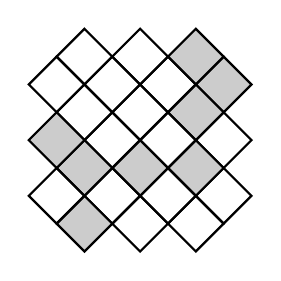
\begin{tikzpicture}[rotate=135]
    
    \( \cell{1}{0}{1.5}{0.5} \);
    \( \cell{1.5}{0}{2}{0.5} \);
    
    \( \cellw{0.5}{0.5}{1}{1} \);
    \( \cell{1}{0.5}{1.5}{1} \);
    \( \cellw{1.5}{0.5}{2}{1} \);
    \( \cellw{2}{0.5}{2.5}{1} \);
    
    \( \cellw{0}{1}{0.5}{1.5} \);
    \( \cell{0.5}{1}{1}{1.5} \);
    \( \cellw{1}{1}{1.5}{1.5} \);
    \( \cellw{1.5}{1}{2}{1.5} \);
    \( \cellw{2}{1}{2.5}{1.5} \);
    \( \cellw{2.5}{1}{3}{1.5} \);
    
    \( \cellw{0}{1.5}{0.5}{2} \);
    \( \cellw{0.5}{1.5}{1}{2} \);
    \( \cell{1}{1.5}{1.5}{2} \);
    \( \cellw{1.5}{1.5}{2}{2} \);
    \( \cellw{2}{1.5}{2.5}{2} \);
    \( \cellw{2.5}{1.5}{3}{2} \);
    
    \( \cellw{0.5}{2}{1}{2.5} \);
    \( \cellw{1}{2}{1.5}{2.5} \);
    \( \cell{1.5}{2}{2}{2.5} \);
    \( \cell{2}{2}{2.5}{2.5} \);
    
    \( \cell{1}{2.5}{1.5}{3} \);
    \( \cellw{1.5}{2.5}{2}{3} \);
    
    \end{tikzpicture}
\end{center}

$$1, 68, 1113, 11616, 104097,\dots$$
\begin{eqnarray*}
    \sum_{n,m\geq 0} \rho(A^{S^*}_{n,m})x^n y^m & = & \\
    & & xy(2 \, x^{5} y - 11 \, x^{4} y^{2} + 9 \, x^{3} y^{3} - 11 \, x^{2} y^{4} + 2 \, x y^{5} \\
    & - & 10 \, x^{4} y + 16 \, x^{3} y^{2} + 16 \, x^{2} y^{3} - 10 \, x y^{4}\\
    & + & x^{4} + 15 \, x^{3} y - 21 \, x^{2} y^{2} + 15 \, x y^{3} + y^{4} - 8 \, x^{2} y - 8 \, x y^{2} \\
    & - & 4 \, x^{2} + 5 \, x y - 4 \, y^{2} + 2 \, x + 2 \, y + 1 ) \\
    & / & {\left(1 - 2 \, x - 2 \, y + x^{2} + x y + y^{2} \right)} {\left(1-x\right)}^{4} {\left(1-y\right)}^{4}
\end{eqnarray*}

\end{document}